\section{Intuition behind Diffusion approximation and BSSRDF formulation}
\label{section:BSSRDF_intuition}
It is clear that for most of the real world problems the analytic solution of the radiative transfer
equation is not possible. Mont Carlo integration gives correct results for the majority of the
complex scenarios but often takes too much time to compute. Especially for highly scattering media,
where the number of events can reach the order of thousands.

Diffusion approximation is particularly suitable method fo solving light simulation in highly
participating media. It gives much faster solution than classic random walks simulation, but has
some applicability limitations.

The first application of the Diffusion Approximation for computer graphics was probably mentioned in
work \cite{Stam1995}. But the main source of the practical solutions for many years was the work
\emph{A Practical Model for Subsurface Light Transport} \cite{Jensen:2001:PMS:383259.383319} Using
of the diffusion approximation is similar to using a normal distribution to estimate the result of
the sum of random variables according to Central Limit Theorem \cite{Glynn1990145}.

Two main conditions apply for reasonable usage of Diffusion Approximation to solve light scattering
in media \cite{wang2007biomedical}:
\begin{itemize}
  \item The number of scattering events is much larger than a number of absorption events. In
  addition to that, after a large number of scattering events the the radiance becomes isotropic.
  \item The mean free scattering path length is much smaller than the characteristic length of the
  change of radiance.
\end{itemize}

In the other words, only high scattering, high albedo materials (with low attenuation) for geometric
objects with with characteristic size much larger than the scattering length can be rendered with
Diffusion Approximation reasonably well.

\begin{figure}[h]
    \centering
    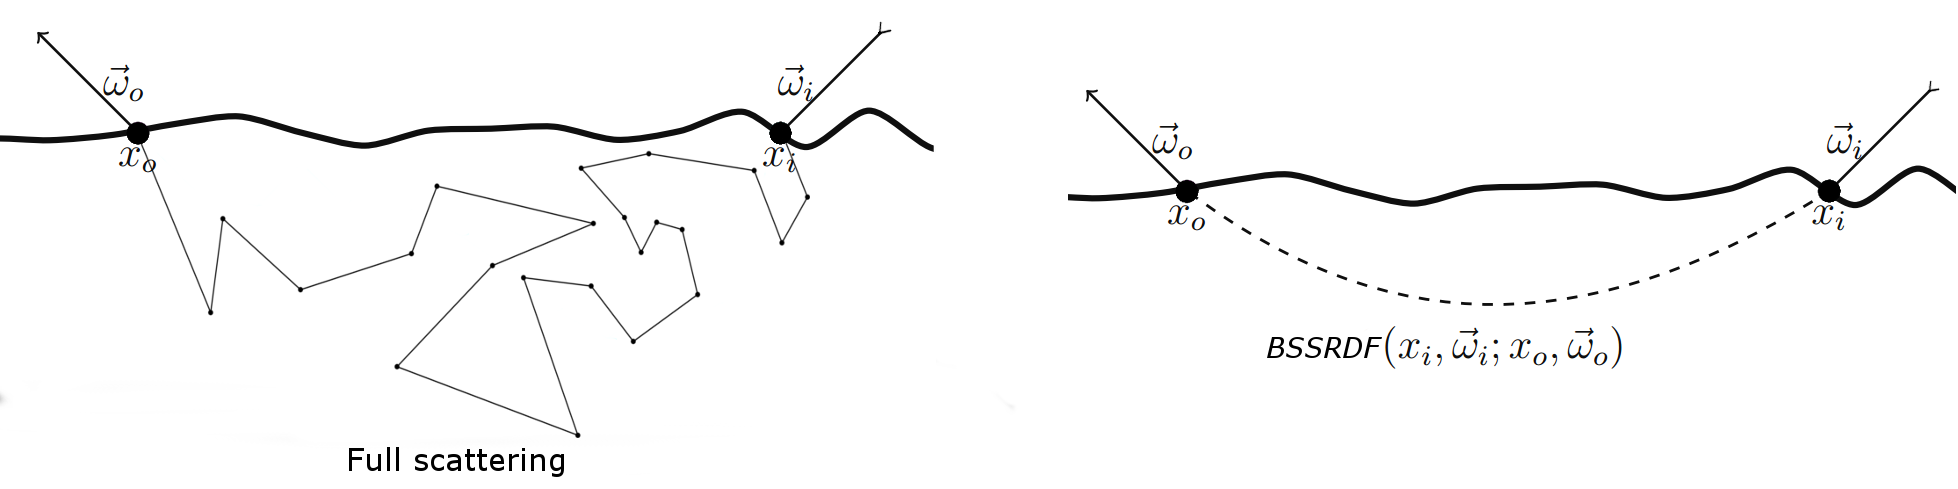
\includegraphics[width=0.9\textwidth]{schemes/bssrdf_path}
    \caption{The full scattering within the media can be approximated by the precomputed attenuation
    function}
    \label{fig:bssrdf_path}
\end{figure}

For practical usage of the Diffusion Approximation the concept of Bidirectional Subsurface
Scattering Reflectance distribution Function is often used \cite{Jensen:2001:PMS:383259.383319}.

The complex and computationally expensive process of simulating the multiple scattering in the media
can be approximated by the function which accounts for the attenuation of the radiance between
incoming and outgoing points on the surface. This approximation usually is computed with the
assumption of the flat semi-infinite surface. This is reasonable a reasonable limitation only if
scattering distance is small with respect to surface curvature and thickness. In the original work
by Jensen \cite{Jensen:2001:PMS:383259.383319} about \emph{Dipole approximation} and many other
improvements like \emph{Multipole} \cite{Donner:2005:LDM:1186822.1073308}, \emph{Quantized
diffusion} \cite{D'Eon:2011:QMR:1964921.1964951} the complex multiple scattering is approximated and
single scattering effects are still computed as a separate term.
